
\begin{flushleft}
	\begin{itemize}
		\item A firewall is a security system that prevent unauthorized access to a computer network. 
		\item \textbf{Firewalls guard traffic at a computer's ports}, where information is exchanged with external devices.
	
	
	\bigskip
	\bigskip
	\begin{figure}[h!]
		\centering
		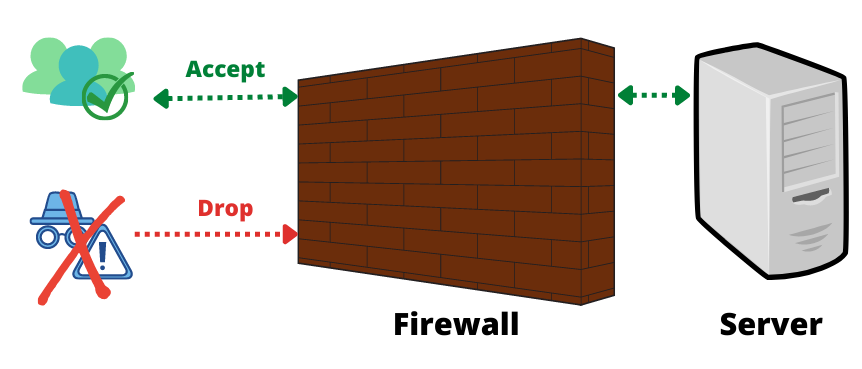
\includegraphics[scale=.5]{content/chapter2/images/firewall.png}
		\caption{Firewall}
		\label{fig:firewall}
	\end{figure}

	\bigskip
	
	\item \textbf{firewalld} is the deamon for firewall in RHEL.
	\item Service unit for this daemon is \textbf{firewalld.service}.
	
	\end{itemize}
	
\end{flushleft}

\newpage

